\vzmstitle{ \bf  Отражение на семействе гипербол}

\vzmsauthor{{Турашова}}{А.\, Н.}

\vzmsinfo(Зеленодольск; {\it annaturaszowa@gmail.com} )

\vzmsauthor{{Хмельницкая}}{А.\, В.}

\vzmsinfo{Зеленодольск;}

\addcontentsline{toc}{section}{Турашова А.Н., Хмельницкая А.В.\dotfill}

Рассмотрим частицу, движущуюся в центрально симметричном поле по гиперболе. Допуская отражение на следе частицы по правилам геометрической оптики, мы определим кривую, состоящую из точек отражения луча, идущего из точки $S$ в точку $P$ на семействе гипербол, задаваемых общей формулой $y= \frac ac + c$, где $a > 0$, $a$ – константа, $c$ – параметр, определяющий конкретную кривую семейства. Ось $OY$ является общей асимптотой этого семейства.

Для простоты описания точку источника $S$ совместим с началом координат точкой $0$.

Точка приёмника $p$ имеет координаты $(0;p)$.

Закон отражения гласит: падающий и отражённый лучи лежат в одной плоскости с нормалью к отражающей поверхности в точке падения, и эта нормаль делит угол между лучами на две равные части.

Обозначим касательный вектор к кривой через \\ $\vec \tau = \{ 1, y_k' \}$, в нашем случае $\vec \tau = \{ 1,- \frac{a}{x^2} \}$.

Построим нормаль $\vec N$ к $\vec \tau$ в точке $M$, используя вектор $\overrightarrow{OM}=\{x,y\}$ и $\overrightarrow{PM}=\{x-p,y\}$:

$$ \vec{N}=\frac{1}{|\overrightarrow{OM}|}\overrightarrow{OM}+\frac{1}{|\overrightarrow{PM}|}\overrightarrow{PM} $$

Тогда условие $(\vec \tau , \vec N)=0$ выражает закон отражения в точке $M$ для луча, идущего из начала координат и попадающего в точку $P$.

В координатах на плоскости из него получим:
\[
\sqrt{x^2+y^2}
\left( p-x+ \frac{ay}{x^2} \right)
=
\sqrt{{(p-x)}^2+y^2}
\left( x - \frac{ay}{x^2} \right)
\]
    --- это соотношение определяет искомую кривую.

Заметим, что множество касательных векторов $\{ \vec \tau_x \}$ для каждого фиксированного $x$ и любого $y$ (а в случае пространства и любого $z$) состоит из параллельных векторов. Используя это свойство для изучения кривой отражения было получено утверждение, носящее общий характер:

\textbf{Теорема~1.} {\it Пусть даны две точки $S$ и $P$ и несрединная прямая $L$, перпендикулярная к отрезку $SP$. Пусть так же дан несобственный пучок прямых, непараллельных отрезку $SP$ и $L$. Существует не более трёх точек пересечения пучка с $L$ --- $M_i$, в которых углы, образуемые отрезками $SM_i$ и $M_iP$ с $L$, равны.}

Приведённая теорема объясняет появление при определённых соотношениях между $a$ и $p$ несвязанного с кривой овала в четвёртой четверти на плоскости и несвязанного с поверхностью эллипсоидального тела в случае трёх измерений. Для трёхмерного случая поверхность отражения задаётся соотношением:
\[
\sqrt{x^2+y^2+z^2}
\left( p-x+ \frac{ay}{x^2} \right)
=
\sqrt{{(p-x)}^2+y^2+z^2}
\left( x - \frac{ay}{x^2} \right)
\]

Поведение кривых, полученных сечением плоскостью \\
$z=z_0$, позволило определить вид поверхности.

Ниже для иллюстрации приводятся сечения $z=0$:

\begin{figure}[h]
\begin{minipage}[h]{0.49\linewidth}
\center{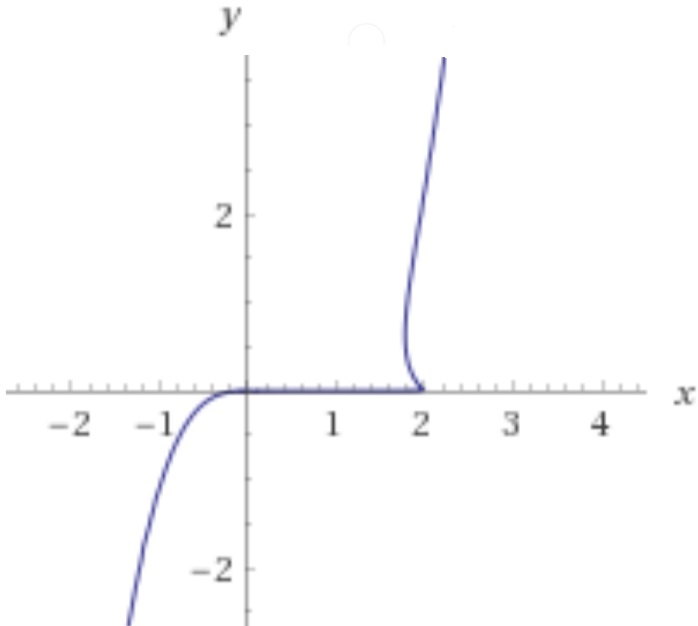
\includegraphics[width=0.85\linewidth]{Turashova_Ris3} \\ Рис.1}
\end{minipage}
\hfill
\begin{minipage}[h]{0.49\linewidth}
\center{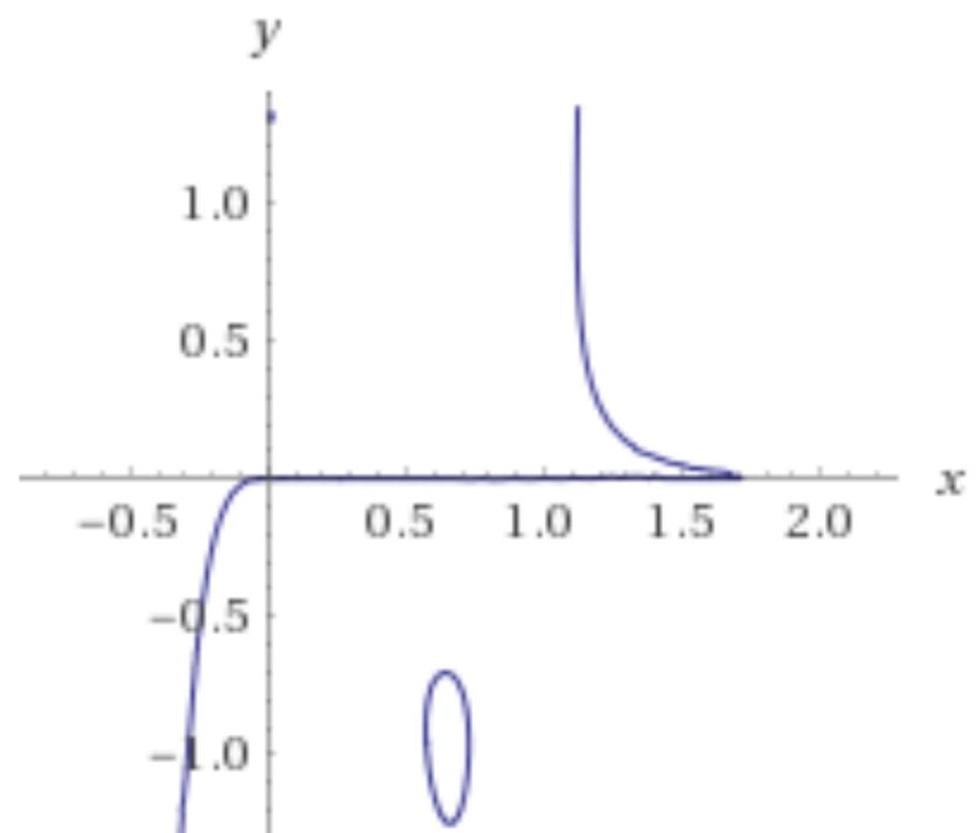
\includegraphics[width=0.89\linewidth]{Turashova_Ris1} \\ Рис.2}
\end{minipage}
\label{ris:image1}
\end{figure}

На левом рисунке кривая при $a=2$, $p=2$, на рисунке справа кривая состоит из двух несвязанных частей  при $a=\frac{1}{13}$ и $p=2$.

\litlist

1. {\it Арнольд В.И.} Теория катастроф. М.: Наука, 1990. — 129 с.

2. {\it Брус Дж., Джиблин П.} Кривые и их особенности. М.: Мир, 1988. — 262 с.
